Historically, computer architecture security relied on processor modes or privilege modes where code was allowed to execute. In these modes, separation of privileges is achieved and often referred to as ``rings'' with ``ring 0'' being the most privileged machine mode where OS kernel code runs and ring 3 being the least privileged user mode where application code runs.

\begin{figure}[htbp]
\centering

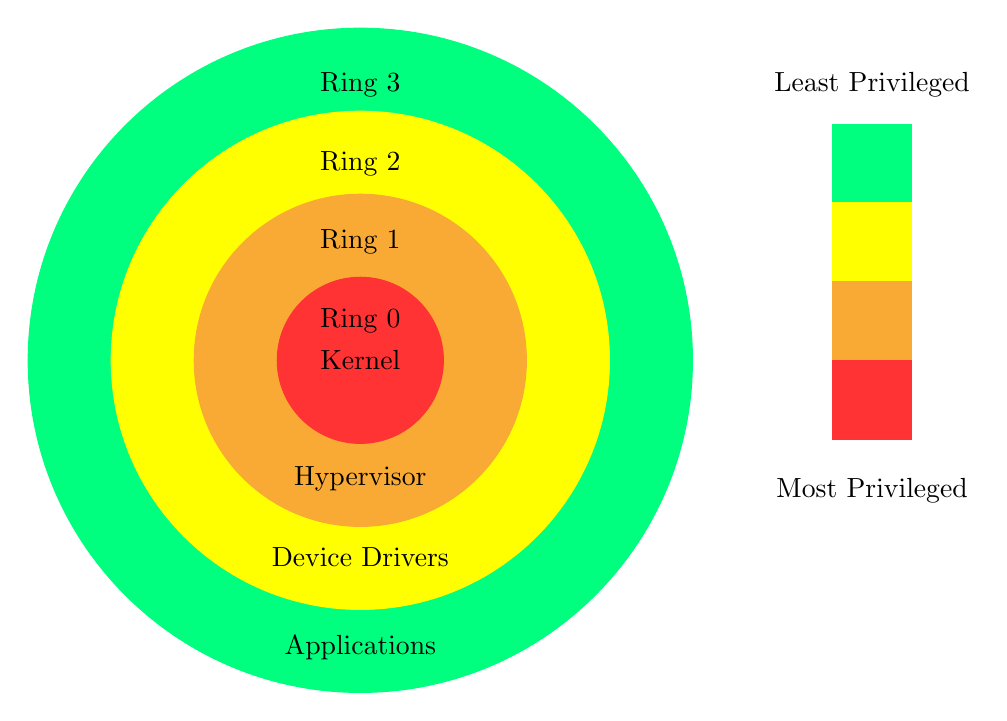
\begin{tikzpicture}

\draw[SpringGreen,fill=SpringGreen] (0,0) circle (120pt);
\draw[Yellow,fill=Yellow] (0,0) circle (90pt);
\draw[YellowOrange!80!,fill=YellowOrange!80!] (0,0) circle (60pt);
\draw[Red!80!,fill=Red!80!] (0,0) circle (30pt);

\node at (0,3.5) {Ring 3};
\node at (0,2.5) {Ring 2};
\node at (0,1.5) {Ring 1};
\node at (0,.5) {Ring 0};
\node at (0,0) {Kernel};
\node at (0,-1.5) {Hypervisor};
\node at (0,-2.5) {Device Drivers};
\node at (0,-3.65) {Applications};

\node at (6.5,3.5) {Least Privileged};

\draw[SpringGreen,fill=SpringGreen] (6,2) rectangle (7,3);
\draw[Yellow,fill=Yellow] (6,1) rectangle (7,2);
\draw[YellowOrange!80!,fill=YellowOrange!80!] (6,0) rectangle (7,1);
\draw[Red!80!,fill=Red!80!] (6,-1) rectangle (7,0);

\node at (6.5,-1.65) {Most Privileged};



\end{tikzpicture}
\caption[Protection Rings]{\textbf{Traditional protection rings for a given processor.}}
\label{fig:rings}
\end{figure}

\noindent Device drivers that run in the rings between ring 0 and ring 3 may have elevated privileges in order to interact with hardware. Virtualization is commonly referred to as running in its own ring at a slightly higher privilege level than even device drivers.  

As applications became more complex, specifically with the advent of large-scale virtualization and the internet, this simple security model broke down as executed code could no longer be trusted, nor its origin verified. The problem of ``secure remote computation'' arises where the data owner must trust not only the software provider, but also the remote computer and infrastructure on which that software is executed. Homomorphic encryption solves the problem of secure remote computation to some extent, however the performance overhead of this transaction limits its application \cite{gentryPhd}.

In an attempt to address the problem of secure remote computation, microprocessor designers have implemented different types of \glspl{tee}, first defined by the Open Mobile Terminal Platform and ratified in 2009 \cite{Confidential2009}. These \glspl{tee} are intended to allow for code and data to reside in a specially provisioned area of memory where the processor can reserve access rights using a given set of rules. The processor will then guarantee the confidentiality and integrity of that region of memory based on the configuration of the system.

In choosing a \gls{tee}, implementers have many complex features to consider before picking a platform. Currently, many resources exist that cover the features and design details of specific \glspl{tee}, however there are few resources that combine this information into one source for comparison. In this thesis, we will examine Intel \gls{sgx}, Arm TrustZone, and RISC-V \gls{pmp} in order to provide a methodology for comparing and evaluating \glspl{tee} by considering these technologies' respective strengths and weaknesses. It is not our goal to characterize one technology as overall superior to another, nor is it our goal to expose fatal flaws that make one technology inherently insecure. Rather, we will describe the properties of a hardware \gls{tee} and illustrate how each technology implements those properties. A comparison of these different implementation details yields a method of evaluating \glspl{tee} for those looking to choose the \gls{tee} that best fits their needs.

These three technologies were chosen for specific reasons. Intel \gls{sgx} is available on most consumer desktop/laptop products, and the technology is now becoming popular on their Xeon line of server/workstation processors. Arm is the defacto architecture used in cell phones and embedded devices. The popularity of these two architectures makes them a natural choice for comparison. The third technology, RISC-V \gls{pmp}, is a newcomer to the stage of \gls{tee} options. We will examine how the more mature technologies have informed choices made by the architects of RISC-V, as they are clearly addressing specific limitations with current technologies. While the method used to examine these technologies will be restricted to those aforementioned three \glspl{tee}, this method can be applied to any \gls{tee}.

The goal of this thesis is to provide hardware implementers with a method for comparative analysis and not to act as a definitive guide to any one of these three technologies. Any hardware implementation details are given only as examples and are not intended to be used in production systems. Furthermore, this thesis is an examination of the hardware and not the many possible software implementations available. As such, while we may discuss firmware and software throughout the thesis, it is not meant to be a guide to properly implementing a complete solution.

This thesis will begin by giving a brief history of \glspl{tee} as well as some of the cryptographic underpinnings of the technology (\autoref{chap:bg}). In considering these topics, we will provide definitions for many of the technologies used in a \gls{tee} in order to constrain ourselves to hardware implementations only. We will then give a detailed analysis of Intel \gls{sgx} (\autoref{chap:sgx}), Arm TrustZone (\autoref{chap:trustzone}), and RISC-V \gls{pmp} (\autoref{chap:pmp}). We will examine how these technologies provide the fundamental properties of a hardware \gls{tee}: code integrity, data integrity, and data confidentiality. Furthermore, we will describe how some of these solutions can provide more advanced features like code confidentiality, authenticated launch, programmability, \gls{attestation}, and recoverability. Lastly we will provide a comparison of the three technologies and their methods for providing the fundamental and advanced properties of a hardware \gls{tee} (\autoref{chap:comp}).